\documentclass[a4paper,onesided,12pt]{report}
\usepackage{styles/fbe_tez}
\usepackage[utf8x]{inputenc} % To use Unicode (e.g. Turkish) characters
\renewcommand{\labelenumi}{(\roman{enumi})}
\usepackage{amsmath, amsthm, amssymb}
 % Some extra symbols
\usepackage[bottom]{footmisc}
\usepackage{cite}
\usepackage{graphicx}
\usepackage{longtable}
\graphicspath{{figures/}} % Graphics will be here

\usepackage{multirow}
%\usepackage{subfigure}
\usepackage{algorithm}
\usepackage{algorithmic}
%\pagestyle{empty}
%\includeonly{introduction} % To only process the given file

% Me added

%\usepackage{subfig}
\usepackage[labelsep=period]{caption}
%\usepackage[subfigure]{tocloft}
%\renewcommand{\cfttabpresnum}{Table }
%\renewcommand{\cftfigfont}{Figure }
\let\belowcaptionskip\abovecaptionskip
\usepackage{color,tabularx,amsmath}
\newcommand\fxbox[1]{\center{\framebox[1.1\width][c]{\strut#1}}}
\newcommand\mxbox[1]{\center{\makebox[1.1\width][c]{\strut#1}}}

%%%%%%%%%%%%%%%%%

\newtheorem{thm}{Theorem}[chapter]
\newtheorem{prop}[thm]{Proposition}
\newtheorem{lem}[thm]{Lemma}
\newtheorem{cor}[thm]{Corollary}
% COVER PAGE
\title{\uppercase{Text Normalization Using Lexical and Contextual Features}}
\turkcebaslik{KELİME VE BAĞLAM BİLGİSİ TEMELLİ METİN NORMALİZASYONU}
\degree{B.S., Computer Science, Istanbul Bilgi University, 2007}
\author{Çağıl Uluşahin Sönmez}
\program{Computer Engineering}
\subyear{2014}

% APPROVED BY PAGE
\supervisor{Assist. Prof.~Arzucan Özgür }
%\cosuperi{Title and Name of Cosupervisor I}
%\cosuperii{Title and Name of Cosupervisor II}
\examineri{Prof.~Tunga Güngör}
\examinerii{Assist. Prof.~Gülşen Cebiroğlu Eryiğit}
%\examineriv{}
%\examinerv{}
\dateofapproval{14.01.2014}

\begin{document}
\setlength{\abovedisplayskip}{1cm}
\setlength{\belowdisplayskip}{1cm}

\pagenumbering{roman}
\makemstitle % M.S. thesis
\makeapprovalpage
\begin{acknowledgements}
I would like to express my deep gratitude to my master thesis supervisor Assist. Prof.~Arzucan Özgür. I have learned many things since I became her student. Her positiveness and encouragement made me complete all those tasks that once seemed impossible. Without her support and guidance I would not be able to complete this thesis successfully.

I would also like to thank my committee members Prof.~Tunga Güngör and Assist. Prof.~Gülşen Cebiroğlu Eryiğit for kindly accepting to be in my thesis committee and for their contribution and support to this work. I also thank my academic advisor Prof.~Fatih Alagöz for his valuable guidance during my master education.

I would like to express my appreciation to Bilgi University Computer Science Department faculty members. Your touch in my path of life and education is priceless, thank you for being a part of my life for such a long time. At each step of my life I always remember and appreciate each and everyone of you, your guidance and support.

I am also thankful for the help and support I have received from my fellow graduate students Arda Çelebi, Haşim Sak, Ahmet Yıldırım and Onur Güngör.

My family is always believed in me and supported me. I am deeply grateful to my mother, father and brother for supporting me and my decisions in each way possible. I would like to thank my mother in law and father in law for their support and love. I consider myself lucky for having such a wonderful family.

At the end I would like express appreciation to my beloved husband Ahter Sönmez who spent sleepless nights with and was always my support in every possible moments. Your advice on both research as well as on my career have been priceless. Words fail to express my gratitude to you.

\end{acknowledgements}
\begin{abstract}
The informal nature of social media text, renders it very difficult to be automatically processed by natural language processing tools. Text normalization, which corresponds to restoring the noisy words to their canonical forms, provides a solution to this challenge.
We introduce an unsupervised text normalization approach that utilizes not only lexical, but also contextual and grammatical features of social text.
The contextual and grammatical features are extracted from a word association graph built by using a large unlabeled social media text corpus.
The graph encodes the relative positions of the words with respect to each other, as well as their part-of-speech tags.
The lexical features are obtained by using the longest common subsequence ratio and edit distance measures to encode the surface similarity among words, and the double metaphone algorithm to represent the phonetic similarity. Unlike most of the recent approaches that are based on generating normalization dictionaries, the proposed approach performs normalization by considering the context of the noisy words in the input text.
%In other words, a noisy word can be normalized to different canonical forms depending on the context of the word in the input text message.
Our results show that it achieves state-of-the-art F-score performance on a standard data set. In addition, the system can be tuned to achieve very high precision without sacrificing much from recall.
\end{abstract}
\begin{ozet}
Sosyal medya metinlerinde kullanılan dilin bozukluğu bu metinleri doğal dil işleme araçları ile otomatik olarak işlemeyi çok zorlaştırmakta. Bu bozuk metinleri düzeltip kitap biçimlerine dönüştürme bir diğer deyişle metin normalizasyonu, bu soruna bir çözüm ortaya koymaktadır.
Bu çalışmada, sosyal metinlerin sözcüksel ve içeriksel özelliklerinin yanısıra dibilgisi özelliklerinden de faydalanılan gözetimsiz bir metin normalizasyonu yaklaşımı sunuyoruz.
İçeriksel ve dilbilgisel özellikler, büyük ve etiketlenmemiş bir sosyal medya derlemi kullanarak oluşturduğumuz kelime ilişkilendirme çizgesi yardımı ile hesaplanıyor. Bu çizge, kelimelerin metin içerisinde birbirleriyle olan konum ilişkilerini ve cümle öğe bilgilerini (part-of-speech) içermektedir.
Sözcüksel özellikleri bulmada kelimelerin en uzun ortak altdizileri ve birbirine dönüşme uzaklıkları gibi yazım benzerlikleri yanısıra double metaphone gibi ses bilimsel benzerlikleri göz önünde bulunduran yöntemlerden faydalanıldı. Yakın zamanda sıkça kullanılan sözlük bazlı çalışmaların aksine, önerdiğimiz yaklaşım metin normalizasyonunu düzeltilecek metnin içeriğini göz önünde bulundurarak uygulamaktadır.
Standart veri seti üzerinde daha önce elde edilmemiş sonuçlara ulaşan sistemimiz farklı parametreler kullanılarak doğruluk~(recall) degerinden ödün vermeden çok daha yüksek duyarlık~(precision) değerlerine ulaşabilmektedir.
\end{ozet}
\tableofcontents
\listoffigures
\listoftables
\begin{symbols}
% The title will be typeset as "LIST OF SYMBOLS".
%
% Use a separate \sym command for each symbols definition.
% First Latin symbols in alphabetical order
\sym{$\text{CL}(o_{i})$}{Candidate List of $o_i$}
\sym{$c_{k}$}{$k^{th}$ Candidate Word/Node for the OOV Token in the Given Input Text}
\sym{$\text{EL}(o_i)$}{Edge List of $o_i$}
\sym{$\text{NL}(o_i)$}{Neighbor List of $o_i$}
\sym{$n_{j}$}{$j^{th}$ Neighbour of the OOV Token in the Given Input Text}
\sym{$o_i$}{$i^{th}$ OOV Token in the Given Input Text}
\sym{$t_{distance}$}{Word Distance Threshold for Contextual Association}
\sym{$t_{edit}$}{Edit Distance Threshold}
\sym{$t_{frequency}$}{Word Frequency Threshold}
\sym{$T_i$}{Tag of a Word}
\sym{$t_{phonetic}$}{Phonetic Edit Distance Threshold}
\sym{ }{}
\sym{ }{}
% Then Greek symbols in alphabetical order
\sym{$\beta$}{Contextual Similarity Minor Score Parameter}
\sym{$\lambda$}{Lexical Similarity Minor Score Parameter}

\end{symbols}

\begin{abbreviations}
 % Abbreviations in alphabetical order
\sym{A}{Adjective}
\sym{C}{Punctuation}
\sym{CMU}{Carnegie Mellon University}
\sym{CWA-Graph}{Contextual Word Association Graph}
\sym{D}{Determiner}
\sym{ED}{Edit Distance}
\sym{G}{Miscellaneous words}
\sym{IV}{In Vocabulary}
\sym{L}{Nominal+verbal}
\sym{LCS}{Longest Common Subsequence}
\sym{LCSR}{Longest Common Subsequence Ratio}
\sym{MT}{Machine Translation}
\sym{N}{Noun}
\sym{NLP}{Natural Language Processing}
\sym{OOV}{Out of Vocabulary}
\sym{P}{Preposition}
\sym{POS}{Part of Speech Tag}
\sym{RT}{Retweet}
\sym{SMS}{Short Messaging Service}
\sym{STT}{Speech To Text}
\sym{URL}{Uniform Resource Locator}
\sym{V}{Verb}
\sym{}{}
\sym{}{}
\sym{}{}
\sym{}{}
\end{abbreviations}


\chapter{INTRODUCTION}
\label{chapter:introduction}
\pagenumbering{arabic}
Within the last decade, the common belief among Internet users that social text has~(or should have) its own lexical and grammatical features has naturally given birth to an Internet language and jargon; which has been steadily growing and evolving ever since~\cite{Choudhury:2007:IMS:1326044.1326048, eisenstein2013bad}. This behavioral preference phenomenon brings another challenge of its own. Not only is the Internet jargon itself growing and evolving in an exponential pace, but also since the beginning of the World Wide Web, the Internet has its own slang. \textit{lol} meaning \textit{laughing out loudly},  \textit{xoxo} meaning \textit{kissing}, \textit{4u} meaning \textit{for you} are among the most commonly used examples of this slang. In addition, these specific forms of informal expressions in social text usually take many different lexical forms when generated by each individual, even though the intended contextual meaning might be the same~\cite{eisenstein2013bad}. In other words, with each different individual the same content is being expressed~(written) in different ways. Due to this unpredicted variety of such expressions, it would be appropriate to call this divergency ``noise'' in social text.

The scope of the problem does not end there. In addition, within the last few years, by the increasing use of mobile devices, social text has now been preferred to be transcribed by using Speech-to-Text~(STT) tools. This text input preference is getting trendier and being used more frequently. The insufficient accuracy of such STT tools brings considerable amount of ``additional noise'' to social text. Tools such as spell checkers and slang dictionaries have been shown to be insufficient to cope with this challenge long time ago~\cite{sproat2001normalization}.

Lastly, when we also consider the usual scarcity of attention when people post messages on social media platforms, the problem of analyzing social text actually goes beyond the reach of human cognitive capacity. The mass usage of such social media platforms makes it impossible to derive analysis results in a limited time scope when processed manually. In addition, most automatic Natural Language Processing~(NLP) tools such as named entity recognizers and  dependency parsers generally perform poorly on social media text~\cite{ritter2010unsupervised}.

Text normalization is a preprocessing step to restore noisy words in text to their original~(canonical) forms~\cite{Han:2011:LNS:2002472.2002520} to make use in NLP applications or more broadly to understand the digitized text better. For example, \textit{talk 2 u later} can be normalized as \textit{talk to you later} or similarly \textit{enormoooos, enrmss} and \textit{enourmos} can be normalized as \textit{enormous}. You can find more examples of normalized text in Table~\ref{tab:sentences}. These noisy tokens are referred as Out of Vocabulary~(OOV) words. The normalization task restores the OOV words to their In Vocabulary~(IV) forms. Table~\ref{tab:normalizations} shows sample OOV words encountered in social media text and their corresponding IV forms.


\begin{table}[hbp]
\caption[Sample tweets and their normalized forms.]{Sample tweets and their normalized forms.}
\label{tab:sentences}
\begin{tabular}{|>{\itshape}p{7cm}|p{7cm}|}
\hline
\underline{Its} a beautiful \underline{nite}, \underline{lukin} for \underline{smth} fun to do, I think I \underline{wanna} be \underline{w} \underline{ma} \underline{frnds}. &
\underline{It’s} a beautiful \underline{night}, \underline{looking} for \underline{something} fun to do, I think I \underline{want to} be \underline{with} \underline{my} \underline{friends}. \\
\hline
\underline{Dnt} always follow \underline{da} crowd, stand \underline{4} \underline{wat} \underline{u} \underline{blv} in. &
\underline{Don't} always follow \underline{the} crowd, stand \underline{for} \underline{what} \underline{you} \underline{beleive} in. \\
\hline
@Cloudy me \underline{tht} go be sad \underline{wen} the hangover hold me \underline{tmr}! &

@Cloudy me \underline{that} going to be sad \underline{when} the hangover hold me \underline{tomorrow}! \\
\hline
I \underline{srsly} need some legend of korra \underline{raight} \underline{nao} \#linplz &
I \underline{seriously} need some legend of korra \underline{right} \underline{now} \#linplz \\
\hline
\underline{Wat} was \underline{tht} for \underline{u} \underline{lil} shit, \underline{dnt} \underline{u} draw on my \underline{enlgand} &
\underline{What} was \underline{that} for \underline{you} \underline{little} shit, \underline{don’t} \underline{you} draw on my \underline{England} \\ \hline
Work \underline{f} a \underline{cos}, not for applause. Live life to \underline{exprss}, not to \underline{imprss} :) & Work \underline{for} a \underline{cause}, not for applause. Live life to \underline{express}, not to \underline{impress} :) \\ \hline
\underline{Hav} guts to say \underline{wat} \underline{u} desire.. \underline{Dnt} beat behind \underline{da} bush!! And \underline{1} \underline{mre} \underline{thng} no \underline{mre} say \textbf{\underline{y}} \underline{r} people's man!! &
\underline{Have} guts to say \underline{what} \underline{you} desire.. \underline{Don’t} beat behind \underline{the} bush!! And \underline{one} \underline{more} \underline{thing} no \underline{more} say \textbf{\underline{you}} \underline{are} people's man!! \\
\hline
There \underline{r} \underline{sm} songs \underline{u} don't want \underline{2} listen \underline{2} \underline{yl} walking \underline{cos} when \underline{u} start dancing \underline{ppl} won't \underline{knw} \textbf{\underline{y}}. &
There \underline{are} \underline{some} songs \underline{you} don't want \underline{to} listen \underline{to} \underline{while} walking \underline{because} when \underline{you} start dancing \underline{people} won't \underline{know} \textbf{\underline{why}}. \\
\hline
\end{tabular}
\end{table}


\begin{table}[tbhp]
\caption{Sample noisy tokens and their normalized forms.}
\centering
\begin{tabular}[h]{|p{3.3cm}|p{3cm}|}
\hline
\textbf{Ill-formed word} & \textbf{Normalization} \\
\hline
ppl & people \\ \hline
tmr &   tomorrow \\ \hline
havent & haven't \\ \hline
soooo &  so \\ \hline
raight & right \\ \hline
raight & alright \\ \hline
cos & because \\ \hline
cos & cause \\ \hline
r  &  are \\ \hline
n &      and \\ \hline
mor &    more \\ \hline
doin &   doing \\ \hline
finge &  finger \\ \hline
tnks  & thanks \\ \hline
makeing & making \\ \hline
friiied &  fried \\ \hline
\end{tabular}
\label{tab:normalizations}
\end{table}

Every OOV word should not be considered for normalization. Social text is continuously evolving with new words and named entities that are not in the vocabularies of the systems~\cite{DBLP:conf/acl/HassanM13}. For example \textit{iPhone, WikiLeaks or tokenizing} have not taken their places in dictionaries yet, so they are OOV words, but they should not be normalized to any other canonical word. In addition, an OOV word can sometimes lexically fit an IV word~(Ex:~\textit{tanks} is both an IV word and an OOV word with the canonical form \textit{thanks}).

The OOV tokens that should be considered for normalization are referred to as ill-formed words. Ill-formed words can be normalized to different canonical words depending on the context of the text. For example, if we look at last two examples in Table~\ref{tab:sentences}, we see that ``y'' is normalized in the first as ``why'' and as ``you'' in the latter. Another example would be ``cos'', it has two common canonical forms ``cause'' and ``because''.
%The task of recognizing which tokens are OOV, and which of those are ill-formed are beyond the scope of this paper.

In~\cite{Choudhury:2007:IMS:1326044.1326048} Choudhury \textit{et al.}~propose that OOV words observed in noisy text can be classified into two groups, unintentional and intentional errors. The unintentional errors are caused by~(i) pressing of the wrong key,~(ii) pressing of a key more than the desired number of times,~(iii) deletion of a character or~(iv) inadequate knowledge of spelling. As for the intentional errors, they can be categorized into four categories: character deletion(``tlk'' for ``talk'', ``msg'' for ``message'', ``tomoro'' for ``tomorrow'', ``mob'' for ``mobile''), phonetic substitution~(``nite'' for ``night'', ``bk'' for ``back'', ``u'' for ``you'', ``m8'' for ``mate''), abbreviations~(``btw'' for ``by the way'', ``kgp'' for ``Kharagpur'') and non-standard usage~(``wanna'' for ``want to'', ``betta'' for ``better'', ``sumfin'' for ``something'', ``b/c'' for ``because'').

In this thesis, we propose a graph based text normalization method that utilizes both contextual and grammatical features of social text. The contextual information of words is modeled by a word association graph that is created from a large social media text corpus. The graph represents the relative positions of the words in the social media text messages and their Part-of-Speech~(POS) tags. The lexical similarity features among the words are modeled using the longest common subsequence ratio and edit distance that encode the surface similarity and the double metaphone algorithm that encodes the phonetic similarity. The proposed approach is unsupervised, which is an important advantage over supervised systems, given the continuously evolving language in the social media domain. The same OOV word may have different appropriate normalizations depending on the context of the input text message. Recently proposed dictionary-based text normalization systems perform dictionary look-up and always normalize the same OOV word to the same IV word regardless of the context of the input text ~\cite{Han:2011:LNS:2002472.2002520,DBLP:conf/acl/HassanM13}. On the other hand, the proposed approach does not only make use of the general context information in a large corpus of social media text, but it also makes use of the context of the OOV word in the input text message. Thus, an OOV word can be normalized to different IV words depending on the context of the input text. Another strength of the proposed system is that it achieves the state-of-the art precision scores, without sacrificing from recall.

\chapter{RELATED WORK}
\label{chapter:related}

Early work on text normalization mostly made use of the noisy channel model. The first work that had a significant performance improvement over the previous research was by Brill and Moore, 2000~\cite{Brill:2000:IEM:1075218.1075255}. They proposed a novel noisy channel model for spell checking based on string to string edits. Their model depended on probabilistic modeling of sub-string transformations. They ran their experiments first using error model in isolation assuming that each word in dictionary has uniform probability. Results showed that longer the word their character level noisy model performs better. When they use a trigram language model that they built using Brown corpus  instead of the uniform distribution, their results improves 22 \%.

Toutanova \textit{et al.}, 2002 improved this approach by extending the error model with phonetic similarities over words~\cite{Toutanova:2002:PMI:1073083.1073109}. They have extended a model that learns rules to predict the pronunciation of a single letter in the word depending on the neighbouring letters in the word. Among those extensions are the using a trigram model phone sequence language model and fourgram vowel sequence language model to re-rank top n results, explicit distinction between middle of the word versus start and end of the word and interpolating the model with the letter based model of Brill and Moore, 2000's~\cite{Brill:2000:IEM:1075218.1075255}. Their extended and combined model substantially reduced the error rate of Brill \textit{et al.}'s model, and performed best at 3-Best results.

Choudhury \textit{et al.}, 2007 developed a supervised Hidden Markov Model based approach for normalizing Short Message Service~(SMS) Texts~\cite{Choudhury:2007:IMS:1326044.1326048}. Cook and Stevenson, 2009 have extended this model by introducing an unsupervised noisy channel model~\cite{Cook:2009:UMT:1642011.1642021}. Rather than using one generic model for all word formations as in Choudhury \textit{et al.}, 2007, they used a mixture model in which each different word formation type was modeled explicitly.

The down side of these methods were:~(i) they did not consider contextual features and~(ii) each of them assumed that tokens have unique normalizations. However, that is not the case for the normalization task. The OOV tokens are ambiguous and without contextual information it is not possible to build models that can disambiguate transformations correctly.

Aw \textit{et al.}, 2006 proposed a phrase-based statistical machine translation~(MT) model for the normalization task~\cite{Aw:2006:PSM:1273073.1273078}. They defined the problem as translating the SMS language to the English language and based their model on two submodels: a word based language model and a phrase base lexical mapping model~(channel model). Their phase base model is an extended noisy channel model which does many word to many word mappings such as ``ysnite'' $\rightarrow$ ''yesterday night''. Their system also benefits from the input context and they argue that the strenght of their model is in its ability to disambiguate mapping as in ``2'' to ``two'' or ``to'' and ``w'' to ``with'' or ``who''. Making use of the whole conversation, this is the closest approach to ours in the mean of contextual sensivity/coverage.

Pennell and Liu, 2011~\cite{pennell2011character} on the other hand, proposed a character level MT system, that is robust to new abbreviations. Their system is a two phase one, on the first phase character level trained MT model used to recognize common used abbreviations and to produce word hypotheses~(making use of CMU lexicon) and in the latter phase a trigram language model is used to choose a hypothesis that fits into context. They also use a reordering moel and a word length penalty while scoring the assigned translation.

Another drawback of supervised models is that they require annotated data, which is not readily available and difficult to create for social media text normalization~\cite{DBLP:conf/emnlp/YangE13}.

More recent approaches handled the text normalization task by building normalization lexicons. Han \textit{et al.}, 2011 developed a two phased model, where they only consider the ill-formed OOV words for normalization~\cite{Han:2011:LNS:2002472.2002520}. First a confusion set is generated using the lexical and phonetic distance features. Later, the candidates in the confusion set are ranked using a mixture of dictionary look up, word similarity based on lexical edit distance, phonemic edit distance, prefix sub-string, suffix sub-string and longest common subsequence~(LCS), as well as context support metrics.

Gouws \textit{et al.}, 2011 on the other hand, proposed an approach that depended highly on user-centric information such as the geological location of the users and the twitter client that the tweet is received from~\cite{Gouws:2011:CBL:2021109.2021113}. Using contextual metrics they modeled the transformation distributions.

Liu \textit{et al.}, 2012 proposed a broad coverage normalization system, which integrates an extended noisy channel model, that is based on enhanced letter transformations, visual priming, string and phonetic similarity~\cite{liu2012broad}. They try to improve the performance of the top $n$ normalization candidates by integrating human perspective modeling.
Yang and Eisenstein, 2013 introduced an unsupervised log linear model for text normalization~\cite{DBLP:conf/emnlp/YangE13}. Their joint statistical approach uses local context based on language modeling and surface similarity. Along with dictionary based models, Yang and Eisenstein's model have obtained a significant improvement on the performance of text normalization systems.

Hassan and Menezes, 2013 generated a normalization equivalence lexicon using Markov random walks on a contextual similarity lattice~\cite{DBLP:conf/acl/HassanM13}. Our approach is different from theirs in several ways. First, our system makes use of the context of the OOV word in the input text, whereas their system is a dictionary-based method that always produces the same normalization to a given OOV word, regardless of its context in the input text. Besides the tokens themselves, we make use of the POS tags in creating the graph as well as the relative positions of the words in the social media text. Hassan and Menezes, 2013 create a bipartite graph, that is relatively more conservative in modeling the context of words. Context of a word is modeled as a window of words of size five. That is, two words to the right of a word and two words to the left of a word constitute the context of a word together. Even if one word is not the same, the context is considered to be different. On the other hand, in our graph, each neighboring token contributes to the context information of a word, which leads to both a higher recall and a higher precision. One other difficulty in their approach that it requires a big clean corpus of English sentences, which is only avaliable commercially.

%We select the most likely IV candidates for an OOV word by considering the strength of associations between the neighbors of the OOV word in the input text, as well as the tokens %in the graph that are strongly associated with these neighbors in the similar contextual and grammatical context.
%One of the biggest difference between our system and theirs is that they make use of a huge clean vocabulary.

%We believe several models such as the morphophonemic similarity, MT, Maximum Likelihood, etc. has their own limits. Higher performance text normalization systems should make %use of contextual analysis.


\chapter{METHODOLOGY}
\label{chapter:method}

%Unsupervised and graph based context aware model:

%In our model we made use of both lexical, contextual and shallow properties of the noisy text which makes use of a weighted token co-occurrence graph.

In this thesis, we propose a graph based approach that models both contextual and lexical similarity features among an OOV word that requires normalization and candidate IV words. A high level overview of our system is shown in Figure~\ref{fig:overview}. An input text is first preprocessed by tokenizing and Part-Of-Speech~(POS) tagging. If the text contains an OOV word, the normalization candidates are chosen by making use of the contextual features which are extracted from a pre-generated directed word association graph, as well as lexical similarity features. Lexical similarity features are based on edit distance, longest common subsequence ratio, and double metaphone distance. In addition, a slang dictionary is used as an external resource to enrich the normalization candidate set. The details of the approach are explained in the following sub-sections.

%%% FIGURE
\begin{figure}[htb]
\begin{center}
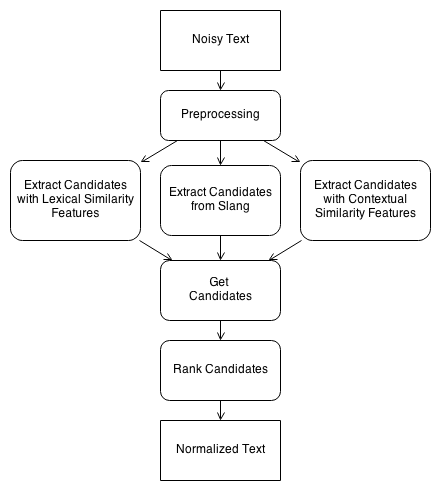
\includegraphics[scale=0.6]{fig/overview}
\caption{High level overview of our system.}
\label{fig:overview}
\end{center}
\end{figure}

\section{Preprocessing}

%Tokenization is the first step in our system. Tokenization is the process of breaking the text into words, numbers, symbols, emoticons After tokenization, next in the pipeline is POS tagging each token using a social media POS tagger. Unlike the normal POS taggers, social media POS taggers~\cite{DBLP:conf/naacl/OwoputiODGSS13}\cite{Gimpel:2011:PTT:2002736.2002747} provide a broader set of tags that is special to the social text. By this extended set of tags we can identify tokens such as discourse markers~(rt for retweets, cont. for a tweet whose content follows up in the coming tweet) or URLs. So that we can process those tokens within their context.

Tokenization is the first step in our system. It is the process of breaking the text into tokens, which are the smallest meaningful elements such as numbers, symbols, and emoticons. After tokenization, the next step in the pipeline is Part-of-Speech~(POS) tagging each token using a POS tagger specifically designed for social media text. Unlike the regular POS taggers designed for well-written newswire-like text, social media POS taggers provide a broader set of tags specific to the peculiarities of social text~\cite{owoputi2013improved,Gimpel:2011:PTT:2002736.2002747}. Using this extended set of tags we can identify tokens such as discourse markers~(e.g.~rt for retweets, cont.~for a tweet whose content follows up in the coming tweet) or URLs. This enables us to better model the context of the words in social media text. A sample preprocessed sentence is shown in Table~\ref{tab:postagged}.

\begin{table}[tbhp]
\caption{Sample tokenized, POS tagged sentence~(L: nominal+verbal, V: verb, D: determiner, N: noun, P: Preposition, A: adjective, C: punctuation).}
\centering
\begin{tabular}{|l|l|l|l|l|l|l|l|l|l|}
\hline
Let's$_{\textcolor{red}{L}}$ & start$_{\textcolor{red}V}$ & this$_{\textcolor{red}D}$ & morning$_{\textcolor{red}N}$ & w$_{\textcolor{red}P}$ & a$_{\textcolor{red}D}$ & beatiful$_{\textcolor{red}A}$ & smile$_{\textcolor{red}N}$ & .$_{\textcolor{red}C}$\\
\hline
\end{tabular}
\label{tab:postagged}
\end{table}
\newpage
As shown in Table~\ref{tab:postags}, after preprocessing, each token is assigned a POS tag with a confidence score between 0 and 1. Later, we use these confidence scores in calculating the edge weights in our context graph. Note that even though the words \emph{w} and\emph{ beatiful} are misspelled, they are tagged correctly by the tagger, with lower confidence scores though.

\begin{table}[htbp]
\caption{Sample POS tagger output obtained by using CMU Ark Tagger~\cite{owoputi2013improved,Gimpel:2011:PTT:2002736.2002747}.}
\begin{minipage}{.5\linewidth}
\begin{tabular}[h]{|l|>{\itshape}l|r|}
 \hline
Token & POS tag & Tag confidence \\
 \hline
with & Preposition & 0.9963 \\
 \hline
a & Determiner & 0.9980 \\
 \hline
beautiful & Adjective & 0.9971 \\
 \hline
smile & Noun & 0.9712 \\
 \hline
\end{tabular}
\end{minipage}
\begin{minipage}{.5\linewidth}
\begin{tabular}[h]{|l|>{\itshape}l|r|}
 \hline
Token & POS tag & Tag confidence \\
 \hline
w & Preposition & 0.7486 \\
 \hline
a & Determiner & 0.9920 \\
 \hline
beatiful & Adjective & 0.9733 \\
 \hline
smile & Noun & 0.9806 \\
 \hline
\end{tabular}
\end{minipage}
\label{tab:postags}
\end{table}

\section{Graph construction}

Contextual information of words is modeled through a word association graph created by using a large corpus of social media text. The graph encodes the relative positions of the POS tagged words in the text with respect to each other. After preprocessing, each text message in the corpus is traversed in order to extract the nodes and the edges of the graph.
%The graph~(See Figure~\ref{fig:graph}) is build using a big dataset of social media text. After preprocessing, we traverse each entry in the dataset and extract nodes and edges.
A node is defined with four properties: \textit{id, oov, freq} and \textit{tag}. The token itself is the \textit{id} field. The \textit{freq} property indicates the node's frequency count in the dataset. The \textit{oov} field is set to True if the token is an OOV word. Following the prior work by Han and Baldwin, 2011 we used the GNU Aspell dictionary~(v0.60.6) to determine whether a word is OOV or not~\cite{Han:2011:LNS:2002472.2002520}. We also edited the output of Aspell dictionary to accept letters other than ``a'' and ``i'' as OOV words. A portion of the graph that covers parts of the sample sentence in Table~\ref{tab:postagged} is shown in Figure~\ref{fig:graph}.

\begin{figure}[htb]
\begin{center}
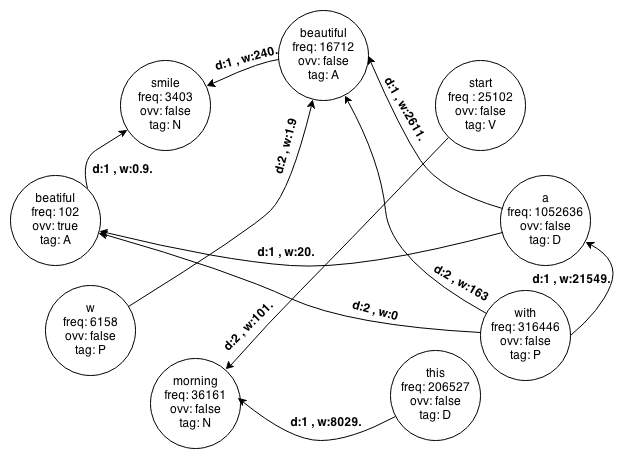
\includegraphics[scale=0.7]{fig/graph}
\caption{Portion of the word association graph for part of the sample sentence in Table~\ref{tab:postagged}.~(d: distance, w: edge weight).}
\label{fig:graph}
\end{center}
\end{figure}

%We define a node with four properties \textit{id, oov, freq, tag}. The token itself plus it's POS tag forms the \textit{id} field. \textit{freq} property indicates the node's frequency count in the dataset. \textit{oov} field is set to True if the token is a OOV word. Following ~\cite{Han:2011:LNS:2002472.2002520} we used GNU Aspell dictionary~(v0.60.6) to determine whether a word is OOV or not.

%In the word-relatedness graph, each node is a unique set of a token and a POS tag~(see Table~\ref{tab:graph}). This helps us to identify the tokens not only lexically and contextually but also~(in terms of POS tags) grammatically.

In the created word association graph, each node is a unique set of a token and its POS tag. This helps us to identify the candidate IV words for a given OOV word by considering not only lexical and contextual similarity, but also grammatical similarity in terms of POS tags. For example if the token \textit{smile} has been frequently seen as a Noun or a Verb, and not in other forms in the dataset~(e.g.~Table~\ref{tab:nodes}), this provides evidence that it is not a good IV candidate as a normalization for an OOV token that has  been tagged as a Pronoun. On the other hand, \textit{smile} can be a good candidate for a Noun or a Verb OOV token, if it is lexically and contextually similar to it.

\begin{table}[hbt]
  \caption{The different nodes in the word association graph representing the token \textit{smile} tagged with different POS tags.}
  \centering
  \begin{tabular}[tc]{|l|l|l|l|}
    \hline

    \textbf{node id} & \textbf{freq} & \textbf{oov} & \textbf{tag} \\
    \hline
    smile & 3 & False & A \\  \hline
    smile & 3403 & False & N \\ \hline
    smile & 2796 & False & V \\ \hline
  \end{tabular}
\label{tab:nodes}
\end{table}

An edge is created between two nodes in the graph, if the corresponding word pair~(i.e.~token/POS pair) are contextually associated. Two words are considered as contextually associated if they satisfy the following criteria:

\begin{itemize}
\item The two words co-occur within a maximum word distance of $t_{distance}$ in a text message in the corpus.
\item Each word has a minimum frequency of $t_{frequency}$ in the corpus.
\end{itemize}

\begin{figure}[htbp]
\begin{center}
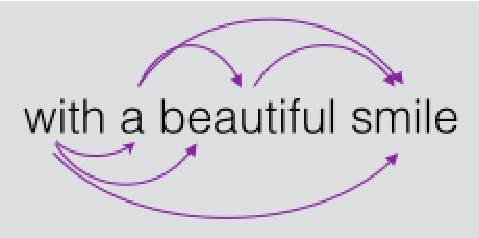
\includegraphics[scale=0.7]{fig/directionality}
\end{center}
\caption{The directionality of the edges is based on the sequence of words in the text messages in the corpus.}
\vskip\baselineskip % Leave a vertical skip below the figure
\label{fig:direction}
\end{figure}
\newpage
The directionality of the edges is based  on the sequence of words in the text messages in the corpus~(see Figure~\ref{fig:direction}). In other words, an edge between two nodes is directed from the earlier seen token towards the later seen token. For example, Table~\ref{tab:edges} and Figure~\ref{fig:edges} show the edges that would be derived from a text including the phrase ``with a beautiful smile''. The \textit{from} property indicates the first word and \textit{to} is the latter in the phrase. The direction and the distance together represent a unique triplet. For each pair of nodes with a specific distance there is an edge with a positive weight, if the two nodes are related. Each co-occurrence of two related nodes increases the weight of the edge between them with an average of the nodes' POS tag confidence scores in the text message considered. If we are to expand the graph with the example phrase shown in Table~\ref{tab:edges}, the weight of the edge with distance $2$ from the node \emph{with$|$P}  to the node  \emph{smile$|$N} would increase by $(0.9963+0.9712)/2$, since the confidence score of the POS tag for the token \emph{with} is  $0.9963$ and the confidence score of the POS tag of the token \emph{smile} is $0.9712$ as shown in Table~\ref{tab:postags}.
%using the given POS tags and accuracies from Table~\ref{tab:postags}, the increase in the weights would be respectively $0.9963+0.9712/2$, $0.998+0.9712/2$ and %$0.9971+0.9712/2$.

\begin{table}[hbt]
  \caption{Example edges extracted from the sample phrase  ``with a beautiful smile''.}
  \centering
  \begin{tabular}[tc]{|l|l|l|l|}
    \hline
\textbf{from} & \textbf{to} & \textbf{distance} & \textbf{weight} \\ \hline
 with$|$P &  smile$|$N & 2 & 89 \\ \hline
 a$|$D & smile$|$N & 1 & 274 \\ \hline
 beautiful$|$A & smile$|$N & 0 & 305 \\ \hline
\end{tabular}
\label{tab:edges}
\end{table}

\begin{figure}[htb]
\begin{center}
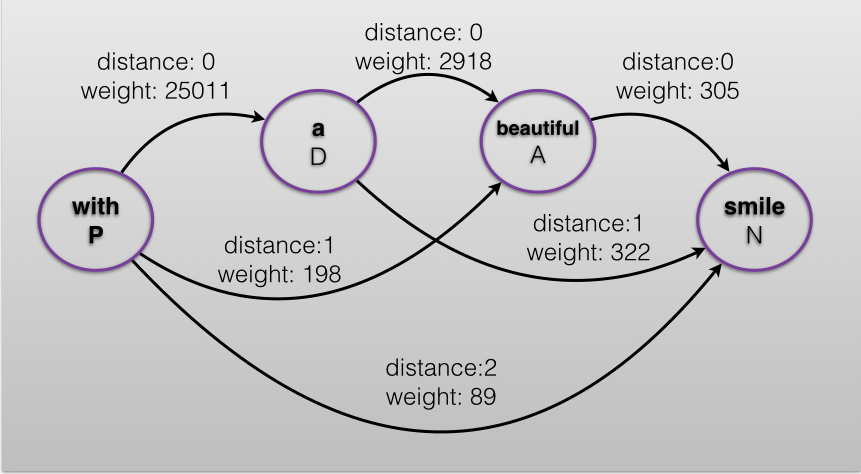
\includegraphics[scale=0.5]{fig/edges}
\caption{Sample nodes and edges from the word association graph.}
\label{fig:edges}
\end{center}
\end{figure}


\section{Graph Based Contextual Similarity}
\label{sec:consim}

Our graph based contextual similarity method is based on the assumption that an IV word that is the canonical form of an OOV word appears in the same context with the corresponding OOV word. In other words, the two nodes in the graph share several neighbors that co-occur within the same distances to the corresponding two words in social media text. We also assume that an OOV word and its canonical form should have the same POS tag.

Given an input text for normalization, the next step after preprocessing is finding the normalization candidates for each OOV token in the input text. For each ill-formed OOV token $o_i$ in the input text, first the list of tokens that co-occur with $o_i$ in the input text and their positional distances to $o_i$ are extracted.  This list is called the neighbor list of token $o_i$, i.e.,  $\text{NL}(o_i)$. Table~\ref{tab:neigh} shows a sample neighbor list for the OOV token beatiful$|$A from the sample sentence in Table~\ref{tab:postagged}.

\begin{table}[hbt]
\caption{Example neighbor list for the OOV node beatiful$|$A.}
\centering
\begin{tabular}{|l|l|l|}
    \hline
    \textbf{id} & \textbf{tag} & \textbf{position} \\
    \hline
    w & P & -2 \\     \hline
    a & D & -1 \\     \hline
    smile & V & 1 \\     \hline
  \end{tabular}
\label{tab:neigh}
\end{table}

For each neighbor node $n_{j}$ in $\text{NL}$, the word association graph is traversed, and the edges from or to the node $n_{j}$ are extracted. The resulting edge list $\text{EL}(o_i)$ has edges in the form of~($n_{j}$, $c_{k}$) or~($c_{k}$, $n_{j}$), where $c_{k}$ is a candidate canonical form of the OOV word $o_i$.
Here the neighbor node $n_{j}$ can be an OOV node, but the candidate node $c_{k}$ is chosen among the IV nodes.
The edges in $\text{EL}(o_i)$ are filtered by the relative distance of $n_{j}$ to $o_i$ as given in the $\text{NL}(o_i)$. Any edge between  $n_{j}$ and $c_{k}$, whose distance is not the same as the distance between $n_{j}$ and $o_i$ is removed.

In addition to distance based filtering, POS tag based filtering is also performed on the edges in $\text{EL}(o_i)$. Each candidate node should have the same POS tag with the corresponding OOV token. For the OOV token $o_i$ that has the POS tag $T_i$, all the edges that include candidates with a tag other than $T_i$ are removed from the edge list $\text{EL}(o_{i})$. Thus, $\text{EL}(o_{i})$ only contains edges where candidate nodes are tagged as $T_i$.

Figure~\ref{fig:edgeWeight} represents a portion from the graph where you can see the neighbours  and candidates of the OOV node ``beatiful''. In the sample sentence in Table~\ref{tab:postagged} there is two OOV token to be normalized, $o_1=w$ and $o_2=beatiful$. The neighbour list of $o_2$, $\text{NL}(o_2)$ includes  $n_1=with$, $n_2=a$ and $n_3=smile$. For each neighbor in the $\text{NL}(o_2)$, the candidate nodes~($c_1=broken$, $c_2=nice$, $c_3=new$, $c_4=beautiful$, $c_5=big$, $c_6=nice$, $c_7=great$) are extracted. As shown in Figure~\ref{fig:edgeWeight}, there are 11 lines representing the edges between the neighbors of the OOV token and the candidate nodes. These are representative edges in the $\text{EL}(o_2)$. Each member of the edge list has the same tag (A for Adjective) as the OOV node ``beatiful'' and each has the same distance to the neighbor node they are connected as the OOV node. We are simply looking for the best replacements using the distance and POS tag properties.

\begin{figure}[htb]
\begin{center}
\includegraphics[scale=0.5]{fig/edgeWeight}
\caption{A portion of the graph that includes the OOV token ``beatiful'', its neighbors and the candidate nodes that each neighbor is connected to. Thick lines shows the edge list with relative weights.}
\label{fig:edgeWeight}
\end{center}
\end{figure}

Each edge in $\text{EL}(o_i)$ consists of a neighbor node $n_j$, a candidate node $c_k$ and an edge weight $\text{edgeWeight}(n_j,c_k)$. The edge weight represents the likelihood or the strength of association between the neighbor node $n_j$ and the candidate node $c_k$. As described in the previous section the edge weights are computed based on the frequency of co-occurrence of two tokens, as well as the confidence scores of their POS tags.

The edge weights of the edges in $\text{EL}(o_2)$ are shown in Figure~\ref{fig:edgeWeight}. The edges that are connected to the OOV neighbor ``w'' have smaller edge weights such as 3,5,26. On the other hand, the edges that are connected to common words have higher edge weight~(e.g.~the edge weight of the edge between nodes ``a'' and ``new'' is 24388). This indicates that those words are non OOV and more common words, and they co-occur very often in the same form (``a new'').

%As shown in Equation~\ref{eq:ew}, we assume that the direction of the edge between two tokens doesn't affect the strength of association between them~(i.e. the edge weight $w$).
Although this edge weight metric is reasonable for identifying the most likely canonical form for the OOV word $o_i$, it has the drawback of favoring words with high frequencies like these common words or stop words. Therefore, to avoid overrated words and get contextually relative candidates, we normalize the edge weight $\text{edgeWeight}(n_j,c_k)$ with the frequency of the candidate node $c_k$ as shown in Equation~\ref{eq:ew_norm}.
\begin{equation}
edgeWeightNormalized(n_j,c_k) = edgeWeight(n_j,c_k) / frequency(c_k)
\label{eq:ew_norm}
\end{equation}

Equation~\ref{eq:ew_norm} provides a metric that captures contextual similarity based on binary associations.
%However we need more than binary relatedness to achive a comprehensive contextual coverage.
In order to achieve a more comprehensive contextual coverage, a contextual similarity feature is built based on the sum of the binary association scores of several neighbors. As shown in Equation~\ref{eq:wscore1}, for a candidate node $c_k$ the total edge weight score is the sum of the normalized edge weight scores $\text{edgeWeightNormalized}(n_j,c_k)$, which are the edge weights coming from the different neighbors of the OOV token $o_i$. We expect this contextual similarity feature to favor and identify the candidates which are (i) related to many neighbors, and (ii) have a high association score with each neighbor.
\begin{equation}
\text{edgeWeightScore}(o_i,c_k) = \sum_{(n_j,c_k) \text{or} (c_k,n_j) \in \text{EL}(o_i)}{\text{edgeWeightNormalized}(n_j,c_k)} \\\\
\label{eq:wscore1}
\end{equation}

Figure~\ref{fig:contextscores} includes the top three candidates sorted by their scores. The candidate node ``beautiful'', $c_4$, has a frequency of 17900. Both three neighbors were paired in the edge list with it with the weights 2, 2918 and 305 respectively~(Figure~\ref{fig:edgeWeight}). After normalizing the edge weight by the frequency of the candidate node  $c_4$, sum of those normalized weights gives us the edge weight score of the candidate node: $\text{edgeWeightScore}(o_2,c_4) = 0.18$.

\begin{figure}[htb]
\begin{center}
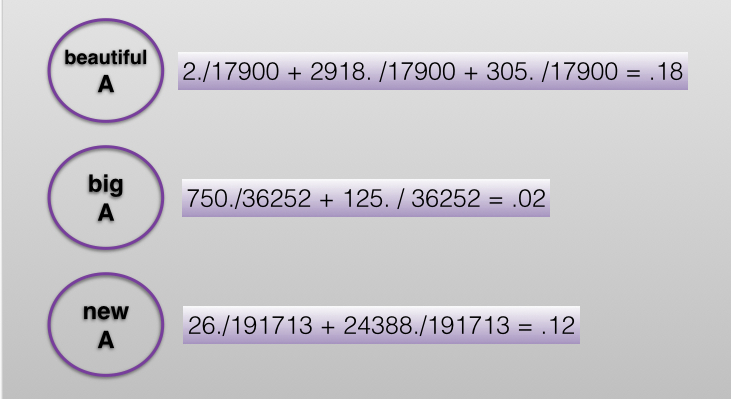
\includegraphics[scale=0.5]{fig/contextScores}
\caption{Candidates for ``beatiful'' sorted by their edge weight scores.}
\label{fig:contextscores}
\end{center}
\end{figure}

Our word association graph includes both OOV and IV tokens, and our OOV detection depends on the spellchecker which fails to identify some OOV tokens that have the same spelling with an IV word. In order to propose better canonical forms, the frequencies of the normalization candidates in the social media corpus have also been incorporated to the contextual similarity feature. Nodes with higher frequencies lead to tokens that are in their most likely grammatical forms.

The final contextual similarity of the token $o_i$ and the candidate $c_k$ is the weighted sum of the total edge weight score and the frequency score of the candidate~(See Equation~\ref{eq:contscore}). The frequency score of the candidate is a real number between 0 and 1. It is proportional to the frequency of the candidate with respect to the frequencies of the other candidates in the corpus. Since the total edge weight score is our primary contextual resource, we may want to favor edge weight score. For that reason we give the frequency score a weight $\beta \leq 1$ to be able to limit its effect to the total contextual similarity score.
\begin{equation}
\text{contextSimScore}(o_i,c_k) = \text{edgeWeightScore}(o_i,c_k) + \beta * \text{freqScore}(c_k)
\label{eq:contscore}
\end{equation}

Hereby, we have the candidate list $\text{CL}(o_{i})$ for the OOV token $o_i$ that includes all the unique candidates in $\text{EL}(o_{i})$ and their contextual similarity scores calculated.

\section{Lexical Similarity}
\label{sec:lexsim}

Following the prior work in~\cite{Han:2011:LNS:2002472.2002520,DBLP:conf/acl/HassanM13}, our lexical similarity features are based on edit distance~\cite{levenshtein1966bcc}, double metaphone~(phonetic edit distance)~\cite{Philips:2000:DMS:349124.349132}, and a similarity function~\cite{Contractor:2010:UCN:1944566.1944588} which is based on Longest Common Subsequence Ratio (LCSR)~\cite{melamed1999bitext}.

Edit distance or in other words Levenshtein distance between two words is defined as the minimum number of single character changes such as insertion, deletion and substitution to convert one word into another. Edit distance has major application in NLP especially in the spell checking.

Double metaphone is an extended word edit distance measure, that not only considers the characters but also the English pronunciations of the words. Like the Soundex algorithm, metaphone algorithm~\cite{philips1990hanging} encodes words. Similar sounding words, in other words phoneticly similar words shares the same keys in these encodings. Metaphone is an extended and more accurate version of Soundex. Double metaphone came out 10 years later than the metaphone and is called the second generation of the metaphone algorithm. Double metaphone produces two keys instead of one, presenting a more valid coverage for some irregularities. % fix and give more detail

The cost function we are using is defined by Contractor \textit{et al.}, 2010~\cite{Contractor:2010:UCN:1944566.1944588}, as the ratio between LCSR of two words and their Edit Distance(ED) cost. You can see the LCSR and cost function shown in Equation~\ref{eq:lcsr} and Equation~\ref{eq:lcsr_cont}. In our case we calculate the similarity cost of the candidate word and the OOV word by dividing their LCSR value to the Edit Distance between them. From now on we will refer to the simCost in Equation~\ref{eq:lcsr_cont} as $\text{LCSR\_ED}$.
\begin{align}
\text{LCSR}(o_j,c_k) &= \frac{length(\text{LCS}(o_j,c_k))}{\text{max}(\text{length}(o_j),\text{length}(c_k))} \label{eq:lcsr}      \\
\text{simCost} (o_j,c_k) &= \frac{\text{LCSR}(o_j,c_k)}{\text{ED}(o_j,c_k)} \label{eq:lcsr_cont}
\end{align}
Following the tradition that is inspired from~\cite{Kaufmann2010} before lexical similarity calculations, any repetitions of characters three or more times in OOV tokens are reduced to two (e.g. \emph{goooood} is reduced to \emph{good}). Then, the edit distance, phonetic edit distance, and $\text{LCSR\_ED}$ between each candidate in $\text{CL}(o_{i})$ and the OOV token $o_i$ are calculated. Edit distance and phonetic edit distance are used to filter the candidates. Any candidate in $\text{CL}(o_{i})$ with an edit distance greater than $t_{edit}$ and phonetic edit distance greater than $t_{phonetic}$ to $o_i$ has been removed from the candidate list $\text{CL}(o_{i})$.

For the remaining candidates, the total lexical similarity score (Equation~\ref{eq:lexscore}) is calculated using $\text{LCSR\_ED}$ and edit distance score\footnote{an approximate string comparison measure (between 0.0 and 1.0) using the edit distance https://sourceforge.net/projects/febrl/}. Similar to contextual similarity score, here we have one main lexical similarity feature and one minor lexical similarity feature. The major lexical similarity feature is $\text{LCSR\_ED}$ and edit distance score is the minor. We assigned a weight $\lambda \leq 1$ to the edit distance score to be able to lower its weight while calculating the total lexical similarity score.
\begin{equation}
\text{lexSimScore}(o_i,c_k) = \text{LCSR\_ED}(o_i,c_k) + \lambda * \text{editDistScore}(o_i,c_k)
\label{eq:lexscore}
\end{equation}

\section{External Score}

 Since some social media text messages are extremely short and contain several OOV words, they do not provide sufficient context, i.e., IV neighbors, to enable the extraction of good candidates from the word association graph. Therefore, we extended the candidate list obtained through contextual similarity as described in the previous section, by including all the tokens in the word association graph that satisfy the edit distance and phonetic edit distance criteria. We also incorporated candidates from external resources, in other words from a slang dictionary and a transliteration table of numbers and pronouns (Table~\ref{tab:transliteral}). If a candidate occurs in the slang dictionary or in the transliteration table as a correspondence to its OOV word, it is assigned an external score of $1$, otherwise it is assigned an external score of $0$.

The transliterations are first used in Gouws \textit{et al.}'s work~\cite{Gouws:2011:CBL:2021109.2021113}. The transliteration table they have built has only numbers in common with ours. Among the token and the transliteration we also have the POS tag information in use which was not available in their system~(Table~\ref{tab:transliteral}).

\begin{table}[ht]
  \caption{Transliteration Candidates extended from~\cite{Gouws:2011:CBL:2021109.2021113}.}
  \centering
    \begin{tabular}[l]{|l|l|l|}
    \hline
    \textbf{token} & \textbf{tag} & \textbf{Transliteration} \\\hline
    1 & ``\$'' & ``one'' \\\hline
    2 & ``\$'' & ``two'' \\\hline
    3 & ``\$'' & ``three'' \\\hline
    4 & ``\$'' & ``for'' \\\hline
    5 & ``\$'' & ``five'' \\\hline
    6 & ``\$'' & ``six'' \\\hline
    7 & ``\$'' & ``seven'' \\\hline
    8 & ``\$'' & ``eight'' \\\hline
    9 & ``\$'' & ``nine'' \\\hline
    0 & ``\$'' & ``zero'' \\\hline
    2 & ``P''  & ``to'' \\\hline
    ``w'' & ``P''  & ``with'' \\\hline
    ``im'' & ``L''  & ``I'm'' \\\hline
    ``cont'' & ``\textasciitilde''  & ``continued'' \\\hline
  \end{tabular}
\label{tab:transliteral}
\end{table}

The external score favors the well known interpretations of common OOV words. However unlike the dictionary based methodologies, our system does not return the corresponding unabbreviated word in the slang dictionary or in the transliteration table directly. Only an external score gets assigned and the candidate still needs to compete with other candidates which may have higher contextual similarities and one of those contextually more similar candidates may be returned as the correct normalization instead of the candidate found equivalent to the OOV word in the slang dictionary (or in the transliteration table).

Some example entries from slang dictionary are shown in Table~\ref{tab:slang}. First and third examples from the table present why choosing directly the equivalent word in the dictionary as the correct normalization is a bad idea. The first word from the table is ``2''. It has widely used as an abbreviation for the word ``too'', however it is also used in place of the word ``to'' as well. Likely ``bc'' can be normalized as ``back'' or ``because'' depending on the context of the sentence. That is why we do not return the corresponding candidate words directly but only increase their score using the external score metric. Other examples from Table~\ref{tab:slang} may give some idea about the overall content of the slang dictionary.

\begin{table}[ht]
  \caption{Some entries from the slang dictionary at http://www.noslang.com/.}
  \centering
    \begin{tabular}[l]{|l|l|}
    \hline
    \textbf{slang} & \textbf{correspondence} \\\hline
    ``2'' & ``too'' \\\hline
    ``acc'' & ``account'' \\\hline
    ``bc'' & `` because'' \\\hline
    ``cr'' & ``can't remember'' \\\hline
    ``dmi'' & ``don't mention it'' \\\hline
    ``dupe'' & ``duplicate'' \\\hline
    ``gfx'' & ``graphics'' \\\hline
    ``h/e'' & ``however'' \\\hline
    ``h4kz0r5'' & ``hackers'' \\\hline
    ``iag'' & ``it's all good'' \\\hline
    ``indie''  & ``independent'' \\\hline
    ``j00'' & ``you'' \\\hline
    ``nemore'' & ``anymore''  \\\hline
    ``y'' & ``why'' \\\hline
  \end{tabular}
\label{tab:slang}
\end{table}

\section{Overall Scoring}

As shown in Equation~\ref{eq:candscore}, the final score of a candidate IV token $c_k$ for an OOV token $o_i$ is the sum of its lexical similarity score, contextual similarity score and external score with respect to $o_i$.
\begin{equation}
\begin{aligned}
\text{candScore}(o_i,c_k) = ~ & \text{lexSimScore}(o_i,c_k) + \text{contextSimScore}(o_i,c_k) \\
& + \text{externalScore}(o_i,c_k)
\end{aligned}
\label{eq:candscore}
\end{equation}

\chapter{EXPERIMENTS}
\label{sec:experiments}

\section{Data sets}
\label{sec:datasets}
We used the LexNorm1.1 dataset~\cite{Han:2011:LNS:2002472.2002520} and Pennell \textit{et al.}'s trigram dataset~\cite{pennell2011character,Pennell2014256} to evaluate our proposed approach. LexNorm1.1 contains $549$ tweets with $1184$ manually annotated ill-formed OOV tokens. It has been used by recent text normalization studies for evaluation, which enables us to directly compare our performance results with results obtained by the recent previous work. Trigram dataset on the other hand is an SMS-like corpus collected from twitter status updates sent via SMS.\@ The dataset does not include the complete tweet text but trigrams from tweets and one OOV word in each trigram is annotated. In total 4661 twitter status messages and 7769 tokens are annotated, previous work has used 80 \% for training and the rest as test set, similarly we used the same 20 \% of the dataset as test set to be able to report our results on the same basis as previous work.

\section{Graph Generation}
We used a large corpus of social media text to construct our word association graph. We extracted 1.5 GB of English tweets from Stanford's 476 million Twitter Dataset~\cite{DBLP:conf/wsdm/YangL11}. The language identification of tweets was performed by using the langid.py Python library~\cite{Lui:2012:LOL:2390470.2390475, Baldwin:2010:LIL:1857999.1858026}.

CMU Ark Tagger, which is a social media specific POS tagger achieving an accuracy of $95\%$ over social media text~\cite{owoputi2013improved,Gimpel:2011:PTT:2002736.2002747}, is used for tokenizing and POS tagging the tweets. Besides the standard POS tags, the POS tagset of the Ark Tagger includes some extra POS tags specific to social media including URLs and emoticons; Twitter hashtags~(\#); and twitter at-mentions~(@). One other tag that is special to social media is ``\textasciitilde'' which means the token is specific to a discourse function of twitter such as \textit{rt, cont.}. Lastly G stands for miscellaneous words including multi word abbreviations like btw~(by the way), nw~(no way), and smh~(somehow).

We made use of these social media specific tags to disambiguate some OOV tokens. For example if OOV token ``cont'' is tagged with the discourse function tag G, we added ``continued'' to the candidate list as an external node.

After tokenization, we removed the tokens that were POS tagged as mention~(e.g. @brendon), discourse marker (e.g. RT), URL, email address, emoticon, numeral and punctuation. The remaining tokens are used to build the word association graph. After constructing the graph we only kept the nodes with a frequency greater than $8$. For the performance related reasons, the relatedness thresholds $t_{distance}$ and $t_{frequency}$  were chosen as $3$ and $8$, respectively. The resulting graph contains $105428$ nodes and $46609603$ edges.

\section{Candidate Set Generation}

While extending the candidate set with lexical features we use ${t_{edit}\leq 2}~\vee~{t_{phonetic} \leq 1}$ to keep up with the settings in Han \textit{et al.}~\cite{Han:2011:LNS:2002472.2002520}. In other words, IV words that are within 2 character edit distance of a given OOV word or 1 character edit distance of a given OOV word under phonemic transcription were chosen as lexical similarity candidates.

\section{Evaluation Metrics}

The main evaluation metrics we have been used in this thesis are precision, recall and f-measure. We run our text normalization method on our two test sets that is introduced in Section~\ref{sec:datasets} and calculated each metric regarding to following definitions.

Precision~(Equation~\ref{eq:precision}) calculates the proportion of correctly normalized words among the keys that we could produce a normalization for. Recall~(Equation~\ref{eq:recall}) shows the amount of correct normalizations over the words that requires normalization. The main metric that we consider while evaluating the performance of our system is F-Measure~(Equation~\ref{eq:f-score}) which is the harmonic mean of precision and recall values.

\begin{equation}
\text{Precision} = \frac{ \text{\# of correctly normalized words}}{ \text{\# of normalized words}}
\label{eq:precision}
\end{equation}

\begin{equation}
\text{Recall} = \frac{\text{\# of correctly normalized words}}{\text{\# of words requires normalization}}
\label{eq:recall}
\end{equation}

\begin{equation}
\text{F-Measure} = \frac{2 * \text{Precision} * \text{Recall} }{\text{Precision} + \text{Recall}}
\label{eq:f-score}
\end{equation}

\chapter{RESULTS AND ANALYSIS}

The results obtained by our proposed Contextual Word Association Graph (CWA-Graph) system on the LexNorm1.1 dataset,
as well as the results of recent studies that used the same data set for evaluation are presented in Table~\ref{tab:results}.

\begin{table}[thb]
  \caption{Results obtained on the LexNorm1.1 dataset.}
  \centering
  \begin{tabular}[t]{|l|c|c|c|}
    \hline
    \textbf{Method} & \textbf{Precision} & \textbf{Recall} & \textbf{F-measure} \\
    \hline
    Han and Baldwin, 2011 & 75.30 & 75.30 & 75.30 \\\hline
    Liu \textit{et al.}, 2011 & 84.13 & 78.38 & 81.15 \\\hline
    Hassan and Menezes, 2013 & 85.37 & 56.40 & 69.93 \\\hline
    Yang \textit{et al.}, 2013 & 82.09 & 82.09 & 82.09 \\\hline
    CWA-Graph   & 85.50 & 79.20 & 82.20 \\
    \hline
  \end{tabular}
  \label{tab:results}
\end{table}

Our CWA-Graph approach achieves the best F-measure ($82.20$) and precision ($85.50$) among the recent previous studies. The high precision value is obtained without compromising much from recall ($79.20$). Our recall is the second best among others. The F-score ($82.09$) obtained by Yang \textit{et al.}'s system is close to ours and the second best F-score, which on the other hand, has a lower precision than our approach~\cite{DBLP:conf/emnlp/YangE13}.


Table~\ref{tab:resultspennell} show the results of our system on the trigram SMS-like dataset. Without any modification to our system or to the parameters, we were able to improve results of Pennell \textit{et al.}~\cite{pennell2011character}.

\begin{table}[thb]
  \caption{Results obtained on the trigram SMS-like dataset.}
  \centering
  \begin{tabular}[t]{|l|c|c|c|}
    \hline
    \textbf{Method} & \textbf{Precision} & \textbf{Recall} & \textbf{F-measure} \\
    \hline
    Pennell \textit{et al.}, 2011 & 69.70 & 69.70 & 69.70 \\\hline
    CWA-Graph   &  \textbf{77.5} & \textbf{67.7}  &  \textbf{72.3} \\\hline
  \end{tabular}
  \label{tab:resultspennell}
\end{table}

The earlier work we compare our system with, assumes that the words to be normalized are given in advance. We also made the same assumption. However unlike other systems\cite{DBLP:conf/emnlp/YangE13,liu2012broad,Han:2011:LNS:2002472.2002520}, our system does not propose a normalization if there are no candidates that are lexically similar, grammatically correct and contextually close enough. For this reason, we managed to achieve a higher precision compared to the other systems. Besides, we made sure that the candidates have a minimum similarity either contextual, lexical, external or some degree of each feature. The results shown at Table~\ref{tab:thresholds} and Table~\ref{tab:thresholdspenn} show that our approach can obtain even higher values of precision by tuning the system threshold (i.e.~the minimum score in Equation~\ref{eq:candscore} to return a token as a candidate canonical form of an OVV token).
\\
\begin{table}[thb]
  \caption{Comparison of results for different threshold values on LexNorm1.1.}
  \centering
  \begin{tabular}[th]{|l|c|c|c|}
    \hline
    \textbf{Threshold} & \textbf{Precision} & \textbf{Recall} & \textbf{F-measure} \\
    \hline
    $\leq$ 1 & 81.2 &	80.8 &	81.0 \\\hline
    1.1 & 81.5 & 80.8 &	81.2 \\\hline
    1.2 & 82.2 &	80.7 &	81.4 \\\hline
    1.3 & 83.7 &	80.2 &	81.9 \\\hline
    1.4 & 84.2 &	80.0 &	82.0 \\\hline
    1.5 & \textbf{85.5} &  \textbf{79.2} &  \textbf{82.2} \\\hline
    1.6 & 88.8	& 75.1	& 81.4 \\\hline
    1.7	& 91.1	& 72.8	& 80.9 \\\hline
    1.8	& 92.3	& 67.6	& 78.0 \\\hline
    2	& 94.1	& 56.4	& 70.5 \\
    \hline
  \end{tabular}
\label{tab:thresholds}
\end{table}

\begin{table}[thb]
  \caption{Comparison of results for different threshold values on trigram dataset.}
  \centering
  \begin{tabular}[th]{|l|c|c|c|}
    \hline
    \textbf{Threshold} & \textbf{Precision} & \textbf{Recall} & \textbf{F-measure} \\
    \hline
    $\leq$ 0.8 &	72.2 & 68.9  &	70.5 \\\hline
    1   & 72.1 & 68.8 &	70.4 \\\hline
    1.1 & 72.6 & 68.8 &	70.7 \\\hline
    1.2 & 73.1 & 68.8 &	70.9 \\\hline
    1.3 & 74.3 & 68.2 & 71.1 \\\hline
    1.4 & 75.5 & 67.8 &	71.4 \\\hline
    1.5 &  \textbf{77.5}  & \textbf{67.7} &  \textbf{72.3} \\\hline
    1.6 & 80.8	& 64.8	& 71.9 \\\hline
    1.7	& 83.3	& 58.4	& 68.7 \\\hline
    1.8	& 86.1	& 52.1	& 64.9 \\\hline
    1.9	& 87.6	& 45.4	& 59.8 \\    \hline
    2.1	& 91.2	& 33.8	& 49.3 \\    \hline
  \end{tabular}
\label{tab:thresholdspenn}
\end{table}

We also test our system on different window sizes. The window size is defined by the number of total neighbours of an OOV word in the given text. When we run our system with a contextual association threshold $t_{distance}=3$, which means two words are considered as contextually associated, if they are within a maximum word distance of 3 in the text, 3 words to the left and 3 words to the right are taken into account for finding contextually similar candidates. For example when we look at the first example in Table~\ref{tab:windowsize}, the $t_{distance}$ is set to 3 and  for the OOV word ``w'', the window size is 7. On the other hand, in the second example, OOV word ``beatiful'' has 3 neighbors on the left but only one neighbour on the right, ending up with a window size 5 when the maximum window size set to 7. Thus the window size is defined by our threshold is only a maximum value, since the OOV word may or may not have enough neighbors to fit the maximum window size. From now on we will refer to maximum window size as just window size.

\begin{table}[thb]
  \caption{Window size examples from our sample sentence from Table~\ref{tab:postagged} for OOV words ``w'' and ``beatiful'' with $t_{distance}=3$ and $t_{distance}=2$.}
  \centering
  \begin{tabular}{|c|*9{c}|}
    \hline
    \textbf{Max window size} & \multicolumn{9}{c|}{\textbf{Sentence}} \\
    \hline & & & & & & & & &  \\ \cline{3-9}

    7 & Let's & \multicolumn{1}{|c}{\underline{start}} & \underline{this} & \underline{morning} & \textbf{w} & \underline{a} & \underline{beatiful} & \multicolumn{1}{c|}{\underline{smile}} & . \\
    \cline{3-9} & \multicolumn{9}{c|}{} \\ [0.01cm]
    \hline  & \multicolumn{9}{c|}{} \\ \cline{5-9}

    7 & Let's & start & this & \multicolumn{1}{|c}{\underline{morning}} &\underline{w} & \underline{a} & \textbf{beatiful} & \multicolumn{1}{c|}{\underline{smile}} & . \\
    \cline{5-9} & \multicolumn{9}{c|}{} \\ [0.01cm]
    \hline  & & & & & & & & & \\ \cline{4-8}

    5 & Let's & start & \multicolumn{1}{|c}{\underline{this}} & \underline{morning} & \textbf{w} & \underline{a} & \multicolumn{1}{c|}{\underline{beatiful}} & smile & . \\
    \cline{4-8} & & & & & & & & & \\ [0.01cm]
    \hline  & & & & & & & & & \\ \cline{6-9}

    5 & Let's & start & this & morning & \multicolumn{1}{|c}{\underline{w}} & \underline{a} & \textbf{beatiful} & \multicolumn{1}{c|}{\underline{smile}} & . \\
    \cline{6-9} & & & & & & & & & \\ [0.01cm]
    \hline
  \end{tabular}
\label{tab:windowsize}
\end{table}

Considering twitter's limit on message lenght and users' tendency of using url and long hastags but short texts, the optimal window size is as expected relatively small. As shown in Table~\ref{tab:windows}, the system achives best results with a window size of 7. This is also the setup we have used for our experiments. With higher window sizes OOV tokens get context information from outer word phrases which include contextually less relevant words. Choosing a smaller window size shortens the execution time, but on the other hand this results in missing some important contextual information.

\begin{table}[htb]
  \caption{Comparison of results for different window sizes.}
  \centering
  \begin{tabular}[th]{|l|c|c|c|}
    \hline
    \textbf{Window size} & \textbf{Precision} & \textbf{Recall} & \textbf{F-measure} \\
    \hline
    3 & 85.3 & 79.0 & 82.0 \\\hline
    5 & 85.6 & 79.1 & 82.2 \\\hline
    7 & \textbf{85.5} &  \textbf{79.2} &  \textbf{82.2} \\\hline
    9 & 85.2 & 79.0  & 82.0 \\\hline
  \end{tabular}
\label{tab:windows}
\end{table}

As described in Section~\ref{sec:consim} and~\ref{sec:lexsim} both contextual and lexical similarity is calculated using two metrics, one major and one minor. The major contextual similarity metric is the edge weight score of the candidates and the major lexical similarity metric is the LCSR which is shown to perform good on finding lexical similarity~\cite{Han:2011:LNS:2002472.2002520,DBLP:conf/acl/HassanM13}. For the minor metrics frequency score and edit distance score we introduced $\beta$ and $\lambda$ parameters respectively to be able to tune their contribution to the overall ranking.

We made experiments with different $\lambda$ and $\beta$ values. In Figure~\ref{fig:lambeta}, performance of the system for different values of $\lambda$ and $\beta$ tested on Lexnorm1.1 can be seen. The experiments showed us $\beta = 0.5$ in the range of  $0.3 \leq \lambda \leq 1$ for Lexnorm1.1 (Figure~\ref{fig:lambeta}) and a narrower range of $0.8 \leq \lambda \leq 1$ for trigram dataset give the best results.

\begin{figure}[htb]
\begin{center}
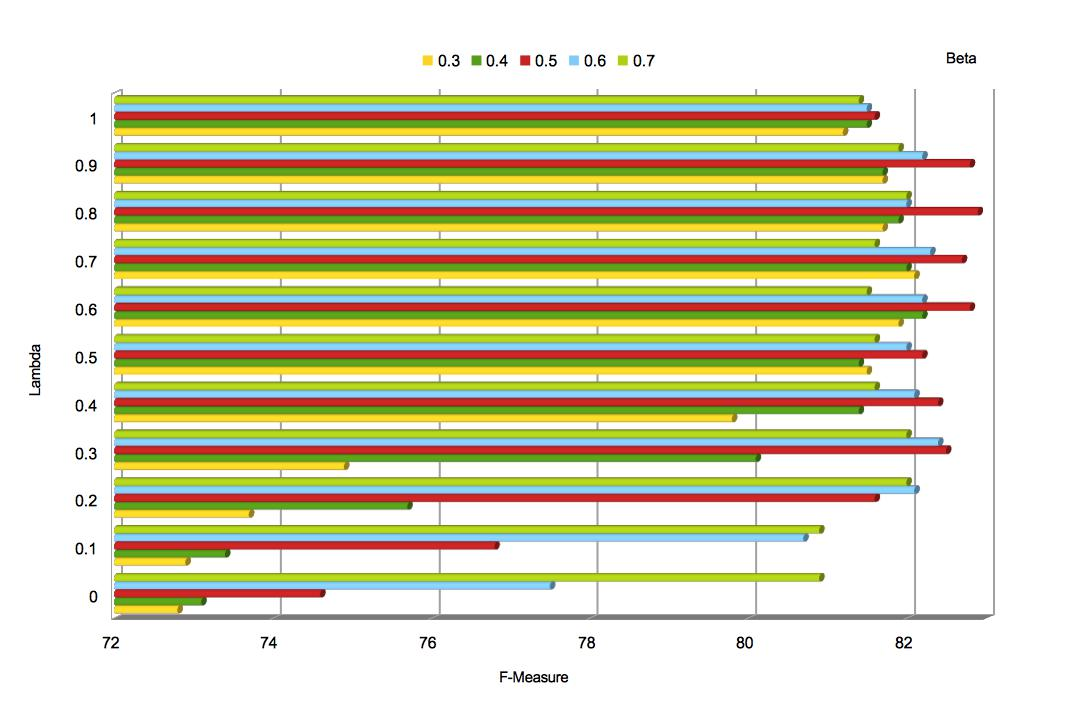
\includegraphics[width=\linewidth]{fig/lambdasandbetas}
\caption{Results on LexNorm1.1 for different $\lambda$ and $\beta$ values.}
\label{fig:lambeta}
\end{center}
\end{figure}

We choose $\beta = 0.5$ and $\lambda = 0.5$ values in our main system. However it is possible to increase these results using higher $\lambda$ values (Figure~\ref{fig:lambdas}).

\begin{figure}[htb]
\begin{center}
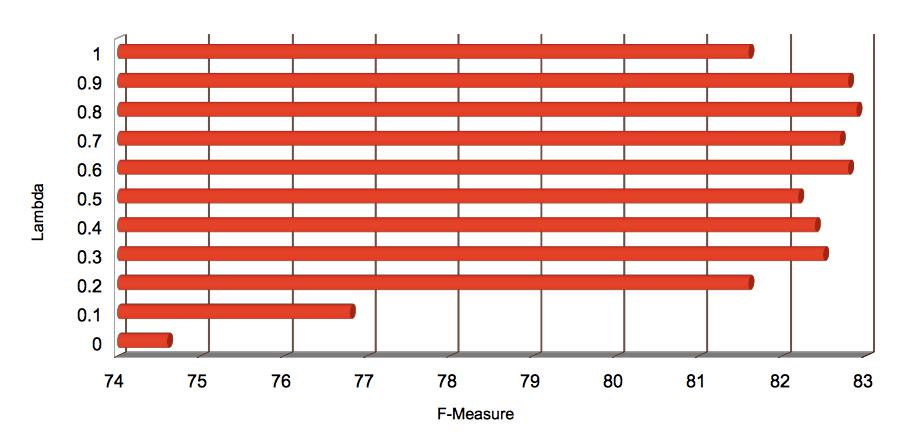
\includegraphics[width=\linewidth]{fig/lambdasforbeta05}
\caption{Results on LexNorm1.1 for $\beta = 0.5$  and $0 \leq \lambda \leq 1.0$.}
\label{fig:lambdas}
\end{center}
\end{figure}

\begin{figure}[htb]
\begin{center}
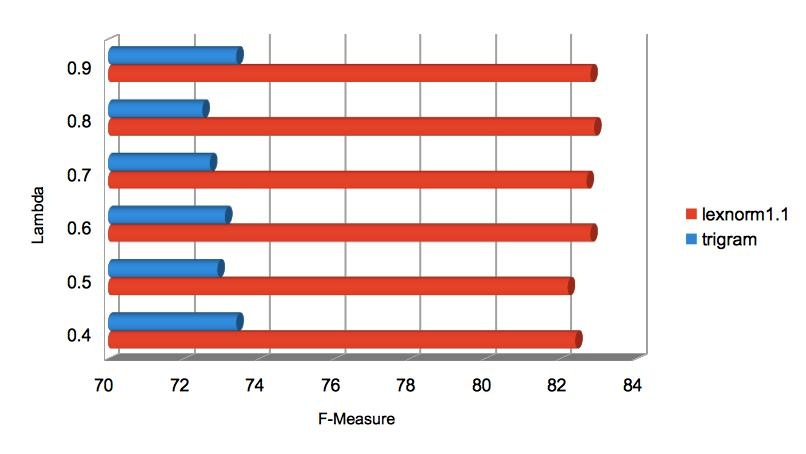
\includegraphics[width=\linewidth]{fig/lambdas_han_penn}
\caption{Results on LexNorm1.1 and trigram dataset for $\beta = 0.5$  and $0.4 \leq \lambda \leq 0.9$.}
\label{fig:lamhanpenn}
\end{center}
\end{figure}

\chapter{CONCLUSION AND FUTURE WORK}

In this thesis, we present an unsupervised graph based approach for contextual text normalization. The proposed approach can analyze grammatical and contextual information from the noisy input text. The task of normalization is highly dependent on understanding and capturing the dynamics of informal nature of noisy text. Our word association graph is built using a large unlabeled social media corpus. It helps to derive contextual and grammatical analysis on both clean and noisy data.

It is important to emphesize the difference between using corpus based contextual information and using contextual information of the input text~(input context). We use corpus based contextual information for building our CWA graph. The graph encodes the context information of words with regard to other words they are contextually associated with. Given an input text that includes an OOV word to normalize, each neighbouring word in the input text gives us context information that we can associate the OOV word with candidates. We use this input based context information to find correct normalization of the OOV word using contextual associations.

It is quite correct to say that using input context to find the correct normalization of OOV words is the major advantage of our system. Many other systems use the corpus based contextual information to find the normalizations, however this approach is lead by statistical information, in other words it finds which IV word the OOV word is normalized to statistically. However, using input context to find normalizations helps us find the correct normalization, not statistically the dominant one.  That way we can use statictical information to connect/associate the words and use input context to associate the correct normalization with the OOV word.

We compared our approach with the recent social media text normalization systems and achieved state-of-the-art precision and F-measure scores. We reported our results on two dataset. The first was the standart text normalization dataset derived from Twitter. Our results on this dataset showed that our system can serve as a high precision text normalization system which is highly preferable as an NLP preprocessing step~\cite{DBLP:conf/acl/HassanM13}. When reaching minimum 10 \% higher precision than other systems, our system can score higher recall than the system with the second best precision score after our system~\cite{DBLP:conf/acl/HassanM13}. It can obviously reach really high precision scores without losing too much from our recall.


The second dataset we tested our approach is a SMS-like trigram dataset. This tests showed that the CWA-Graph can perform good on SMS data as well. However the trigram nature of the dataset resulted in input texts which are very limited with regard to contextual information. The experiments we ran on this dataset with different minor metric parameters also showed that the dataset is dependent on lexical similarity metrics. The reason behind this bias is the lack of enough contextual information. On the other hand our system performed quite good using this contextual information even though it is limited because the SMS-like nature of the dataset makes it rich on abbreviations. Abbreaviations are difficult to normalize using only lexical features due to the higher edit distance values. Not filtering candidates with higher degree of lexical distances results in huge lists of candidates~\cite{Han:2011:LNS:2002472.2002520}, which makes it harder to choose right candidates. Overall although being around 8 \% lower than standard data set, the performance of our system on SMS-like data is reasonably high.

The two lexical metrics we have been used have been already shown to perform good on normalization task~\cite{Han:2011:LNS:2002472.2002520,DBLP:conf/acl/HassanM13}. However LCSR was a better approach than the simple edit distance score. Depending on this assumption we choose one major metric for both lexical and contextual similarity calculations and lowered the weight of the second metric~(minor metric). When we run tests with different weightings of the minor metrics, the results showed us three important output.
\begin{itemize}
\item The minor metrics are increasing the performance of the system.
\item The system performs best for the values of weights that are closer to 0.5.
\item The system does not perform better when weights are 1 than they are smaller than 1.
\end{itemize}

That showed that lowering the contribution of these minor metrics increases the overall performance of normalization task both contextually and lexically. Whereas the absence of these minor metrics or making them also the major metrics by assigning the weights as 1 leads to loss in performance.

Except for the double metaphone algorithm that encodes the phonetic similarities among words in English, the proposed approach is highly language independent. The system does not require a clean corpus, to build the whole system publicly avaliable social text and tools are enough.

As future work, OOV detection can be added to the system. A graph based approach can be proposed to detect OOV words or overall performance of system to decide which word to normalize and which word not to can be increased.

Another task to do next could be integrating the normalization system into an application. This way we can measure how well the normalization system performs as a preprocessing step in NLP applications.

Last item in our future work list is adopting the system to be able to work on another language. This way we can test the advantages our system on other languages and difficulties performing normalization task in a language other than English.


% \nocite{NewEntry1,NewEntry2,NewEntry3,NewEntry4,NewEntry5,
% NewEntry6,
% NewEntry7,NewEntry8,NewEntry9,NewEntry10,NewEntry11,NewEntry12}
%\appendix
%\chapter{APPLICATION}
%The appendices start here.
%\cite{*}
%\bibliographystyle{plain}
\bibliographystyle{styles/fbe_tez_v11}
\bibliography{sentic}

\end{document}